\documentclass[a4paper,12pt]{article}
\usepackage{graphicx}
\usepackage{enumerate}
\usepackage{geometry}
\usepackage{times}
\geometry{legalpaper, portrait, margin=.75in}

\begin{document}

\begin{flushright}

\vspace{1.1cm}

{\bf\Huge Lab 2}

\rule{0.25\linewidth}{0.5pt}

\vspace{0.5cm}
%Put Authors
Justin Ely
\linebreak
\newline
%Put Author's affiliations
\footnotesize{615.202.81.FA15 Data Structures \\}
\vspace{0.5cm}
% Date here below
27 October, 2015
\end{flushright}

\noindent\rule{\linewidth}{1.0pt}

%%%%%%%%%%%%%%%%%%%%%%%%%%%%%%%%%%%%%%%%%%%%%%%%%%%%%%%%%%

\section{Comments}

\subsection{Iterative}


%%%%%%%%%%%%%%%%%%%%%%%%%%%%%%%%%%%%%%%%%%%%%%%%%%%%%%%%%%

\section{Design}

\subsection{Limitations}
The Matrix class is limited to only integer types of the standard int precision.  A matrix, in abstract, is not limited to integers.  
For the current purposes, the required input was limited to integers, so only an integer constructor and methods were added. 

The Determinate method, however, is limited by long-integer precision.  For orders beyond 6, development quickly showed that
the standard int precision wasn't sufficient.  Therefore a long-int precision was implemented instead.  However, this still limits the final
determinate calculation, though to a higher value than ints.  

\subsection{Enhancements}
Though not entirely an enhancement, the given requirements only specify a maximum matrix order of 6, and my design
allows an arbitrary matrix size.  This arbitrary size is only realistically only useful up to order $\sim$10, after which the evaluation time
becomes prohibitive. 

Arguably an enhancement, the main driver's file parsing is able to handle very poorly formatted input matrices.  The only requirement 
is for a first integer $(n)$ followed by $n^2$ integers.  The first integer is evaluated as the matrix order, and the following values are 
inserted in row-major order.  This means they could be input all as a single line, each on newlines, or anything in-between so long as
the number of values is equal to $o^2$.  This is only {\it arguably} an enhancement as, in certain circumstances, this could be seen as
a limitation in not checking for properly formatted row/column data.  For the current requirements, this was deemed not a concern, and in
many implementations such a flexible input format could be a benefit.

An additional enhancement was the implementation of a Print() method for the matrix.  Very useful for debugging and 
verification, the simple method was perhaps the most useful addition during development.


%%%%%%%%%%%%%%%%%%%%%%%%%%%%%%%%%%%%%%%%%%%%%%%%%%%%%%%%%%

\section{Efficiency}
The efficiency of the determinate calculation is limited most by the method employed to find the minor element, as the 
random access of the array implementation allows O(1) operations for other two terms of the Determinate calculation.
The Minor method, needs to iterate over every element of the input matrix, copying it's value into the output matrix (while 
skipping the row, column for which the matrix is to be determinate).  Thus, a single Minor() evaluation is of $O(n^2)$, but a 
recursive call to Determinate will need to calculation the minor N times. 

To test the real-world complexity of the determinate calculation, timing functionality was added to test the actual time required
to calculate the determinate of each order. The results, as well as a fit to the data, can be seen in Figure 1.  From this analysis, we
can see that the time-complexity is exponential, $O(10^n)$.  For the system used for testing (2.8Ghz Intel Core i7), the determinate of 
the matrix order 13 took $\sim$30 minutes to evaluate.

\begin{figure}[h]
    \centering
    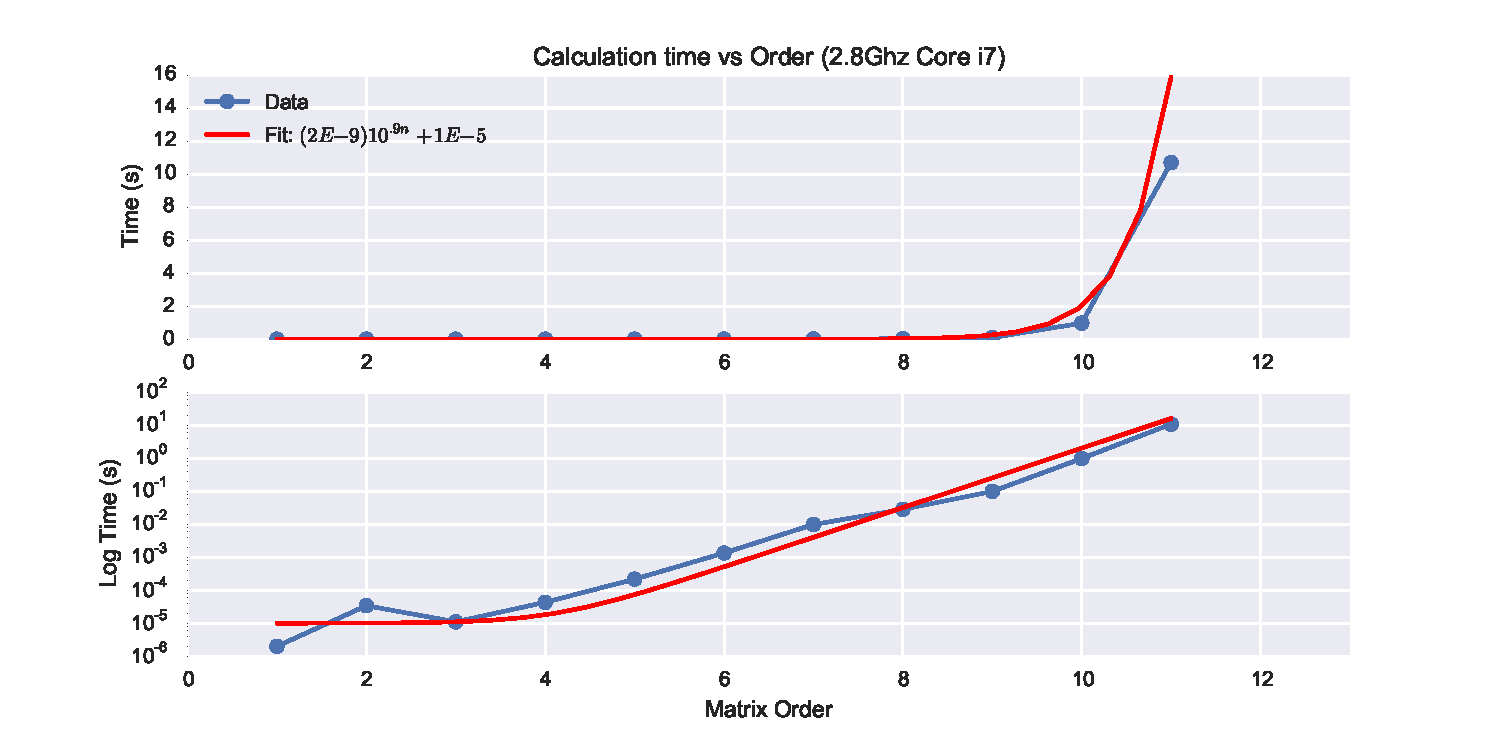
\includegraphics[width=.9\textwidth]{time_complexity.pdf}
    \caption{Time complexity of the determinate method.  Note the variation in behavior at low-numbers.}
    \label{fig:mesh1}
\end{figure}

Real-world evaluation of space complexity was difficult to evaluate directly, so a theoretical calculation was done instead.  
\begin{figure}[h]
    \centering
    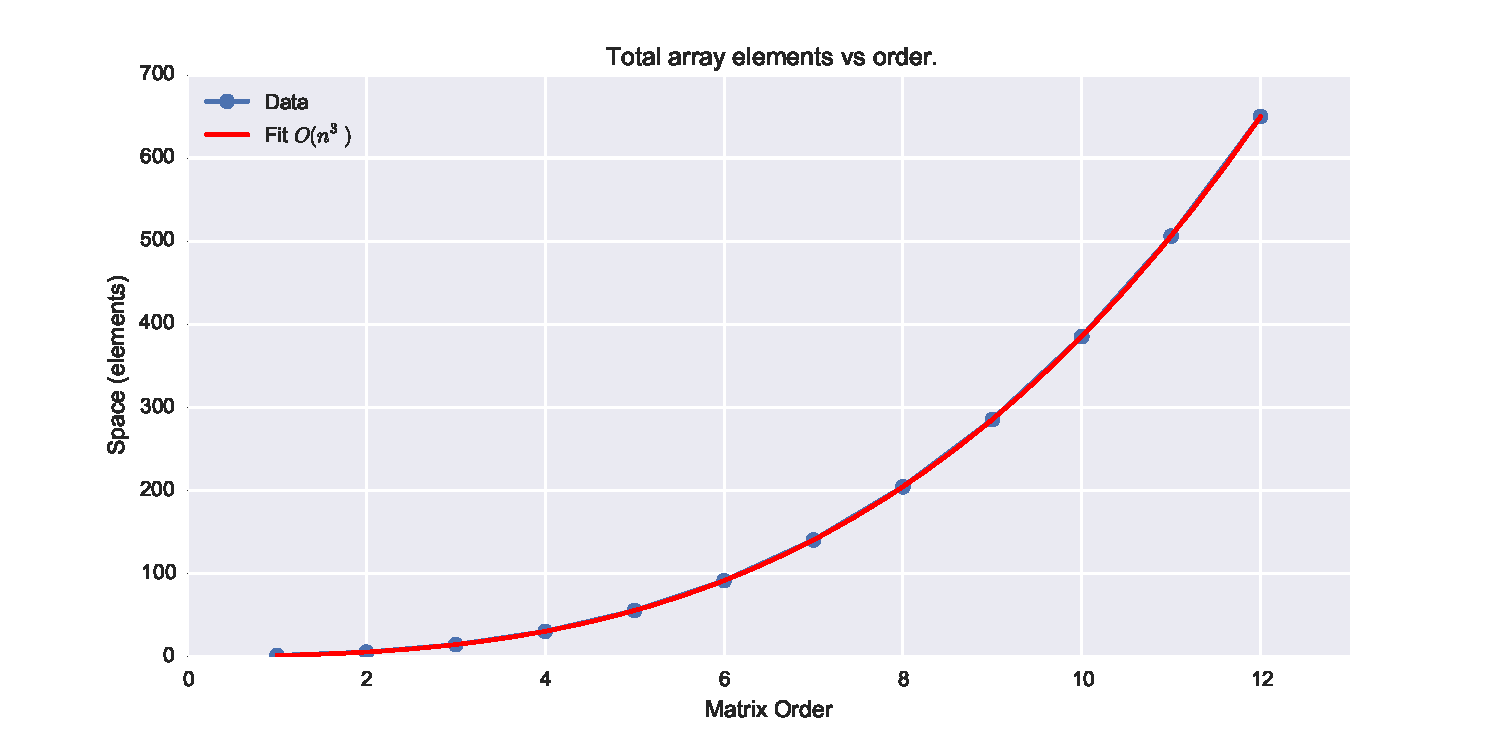
\includegraphics[width=.9\textwidth]{space_complexity.pdf}
    \caption{Space complexity of the determinate method.  The behavior shown is calculated, not observed, and is well fit by
     an $O(n^3)$ polynomial.}
    \label{fig:mesh1}
\end{figure}


%%%%%%%%%%%%%%%%%%%%%%%%%%%%%%%%%%%%%%%%%%%%%%%%%%%%%%%%%%

\section{What I learned}

\subsection{Complaints}

%%%%%%%%%%%%%%%%%%%%%%%%%%%%%%%%%%%%%%%%%%%%%%%%%%%%%%%%%%

\section{Next time}
In a future implementation, i'd like to add more methods to the matrix object to support common operations.  Operations such
as transpose, add, subtract, multiply, and divide are commonly used methods that would make the matrix much more useful
to en end-user.  

Additionally, allowing floating-point numbers in the matrix would be a considerable advantage to use.

Perhaps the most useful change I'd like to make would be to the Minor method itself.  The algorithm implemented here is 
very brute-force, with no attempt at optimization, and is very slow for even moderately sized matrices.  Next time, I'd devote 
more effort into researching and implementing alternate Minor algorithms that have better time efficiency.


%%%%%%%%%%%%%%%%%%%%%%%%%%%%%%%%%%%%%%%%%%%%%%%%%%%%%%%%%%

\end{document}
